\subsection{Funzionalità previsione media}
\begin{figure}[H]
	\centering
	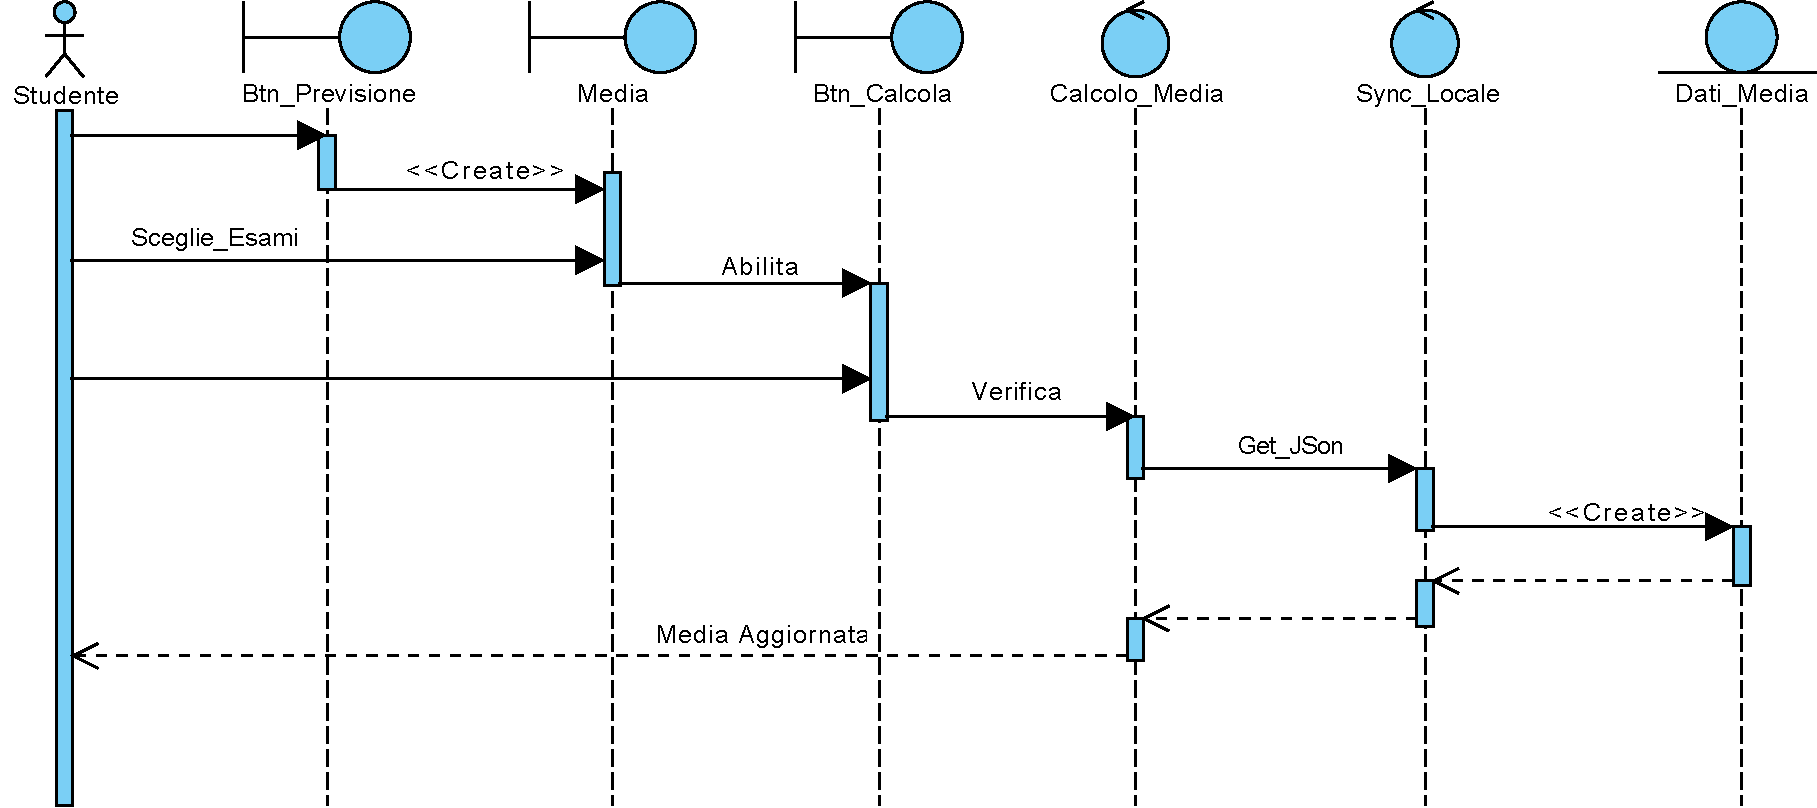
\includegraphics[width=0.9\textwidth]{imgs/gruppo3/sequence-media-valori-validi.pdf}
	\caption{sequence simulazione media}
	\label{fig:seq1-media}
\end{figure}

\begin{figure}[H]
	\centering
	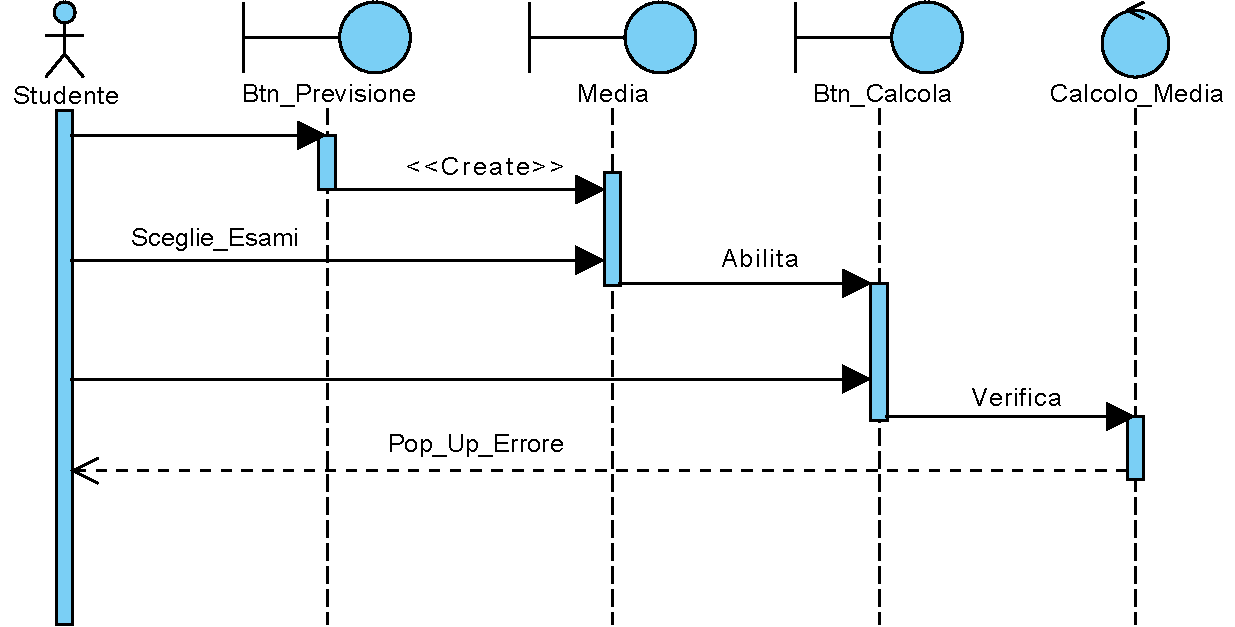
\includegraphics[width=0.9\textwidth]{imgs/gruppo3/sequence-media-valori-non-validi.pdf}
	\caption{Sequence simulazione media con valori non validi o vuoti}
	\label{fig:seq2-media}
\end{figure}

\begin{figure}[H]
	\centering
	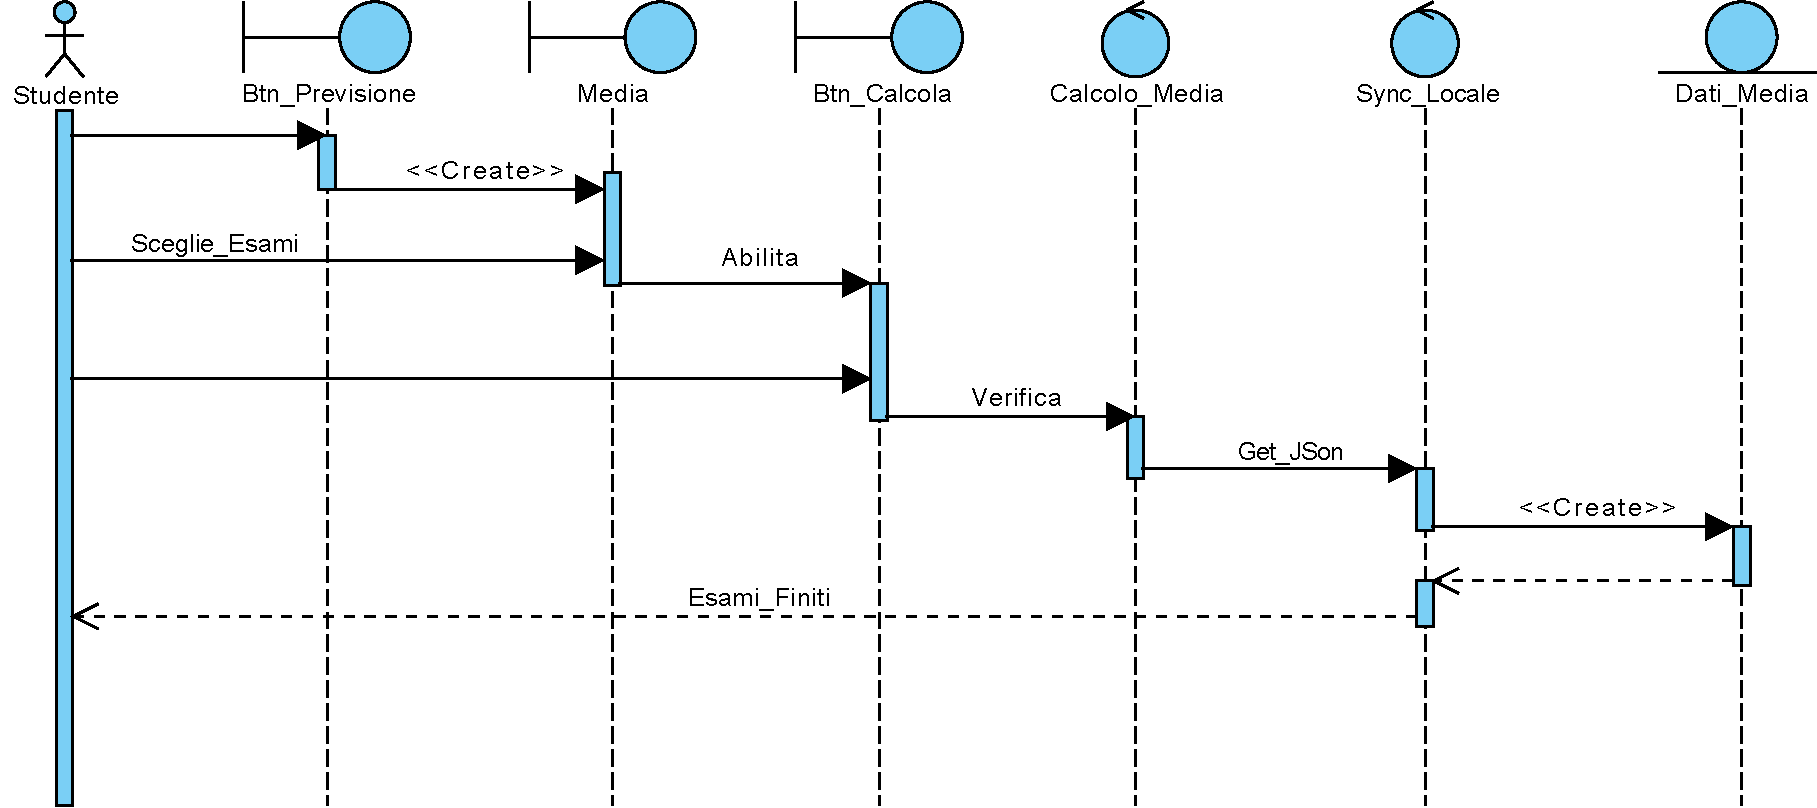
\includegraphics[width=0.9\textwidth]{imgs/gruppo3/sequence-media-esami-finiti.pdf}
	\caption{Sequence simulazione media con esami finiti}
	\label{fig:seq3-media}
\end{figure}

\clearpage